\documentclass{article}\usepackage[]{graphicx}\usepackage[]{color}
% maxwidth is the original width if it is less than linewidth
% otherwise use linewidth (to make sure the graphics do not exceed the margin)
\makeatletter
\def\maxwidth{ %
  \ifdim\Gin@nat@width>\linewidth
    \linewidth
  \else
    \Gin@nat@width
  \fi
}
\makeatother

\definecolor{fgcolor}{rgb}{0.345, 0.345, 0.345}
\newcommand{\hlnum}[1]{\textcolor[rgb]{0.686,0.059,0.569}{#1}}%
\newcommand{\hlstr}[1]{\textcolor[rgb]{0.192,0.494,0.8}{#1}}%
\newcommand{\hlcom}[1]{\textcolor[rgb]{0.678,0.584,0.686}{\textit{#1}}}%
\newcommand{\hlopt}[1]{\textcolor[rgb]{0,0,0}{#1}}%
\newcommand{\hlstd}[1]{\textcolor[rgb]{0.345,0.345,0.345}{#1}}%
\newcommand{\hlkwa}[1]{\textcolor[rgb]{0.161,0.373,0.58}{\textbf{#1}}}%
\newcommand{\hlkwb}[1]{\textcolor[rgb]{0.69,0.353,0.396}{#1}}%
\newcommand{\hlkwc}[1]{\textcolor[rgb]{0.333,0.667,0.333}{#1}}%
\newcommand{\hlkwd}[1]{\textcolor[rgb]{0.737,0.353,0.396}{\textbf{#1}}}%
\let\hlipl\hlkwb

\usepackage{framed}
\usepackage{changepage}
\usepackage{amsfonts}
\makeatletter
\newenvironment{kframe}{%
 \def\at@end@of@kframe{}%
 \ifinner\ifhmode%
  \def\at@end@of@kframe{\end{minipage}}%
  \begin{minipage}{\columnwidth}%
 \fi\fi%
 \def\FrameCommand##1{\hskip\@totalleftmargin \hskip-\fboxsep
 \colorbox{shadecolor}{##1}\hskip-\fboxsep
     % There is no \\@totalrightmargin, so:
     \hskip-\linewidth \hskip-\@totalleftmargin \hskip\columnwidth}%
 \MakeFramed {\advance\hsize-\width
   \@totalleftmargin\z@ \linewidth\hsize
   \@setminipage}}%
 {\par\unskip\endMakeFramed%
 \at@end@of@kframe}
\makeatother

\definecolor{shadecolor}{rgb}{.97, .97, .97}
\definecolor{messagecolor}{rgb}{0, 0, 0}
\definecolor{warningcolor}{rgb}{1, 0, 1}
\definecolor{errorcolor}{rgb}{1, 0, 0}
\newenvironment{knitrout}{}{} % an empty environment to be redefined in TeX

\usepackage{alltt}
\IfFileExists{upquote.sty}{\usepackage{upquote}}{}

\usepackage{apacite}

\begin{document}

\section{Introduction}
Predicting the outcomes of prospective events is the object of much scientific
inquiry and the basis for many decisions both public and private. Because 
predictions of the future can almost never be precise, it is usually desirable
that a level of uncertainty be attached to any prediction. In recent years, it
has become increasingly desirable that forecasts be probabilistic in order to 
account for uncertainty in predicted quantities or events 
\cite{gneiting2014probabilistic}. Specific problems for 
which probabilistic forecasts is used include weather forecasting
\cite{baran2018combining}, economics \cite{groen2013real} and disease outbreaks
\cite{yamana2016superensemble}.

A probabilistic forecast is a forecast to which probabilities are assigned to 
various possible outcomes. There are a number of ways the probabilities or 
uncertainty may be represented. A common representation is either a continuous 
or
discrete parametric distribution function (a pdf or pmf). Much of the literature 
on calibration, sharpness and scoring of a forecast pertains to parametric 
distribution forecasts (see for example 
\cite{gneiting2007probabilistic},
\cite{gneiting2013combining} \cite{baran2018combining}).
Other common representations include samples \cite{krueger2016probabilistic}, 
discretized bins 
and quantile or interval type forecasts \cite{taylor2021evaluating} 
\cite{bracher2021evaluating}. Each representation may be more or less 
appropriate than the others for a given problem but knowing how to interpret, 
score and contruct ensemble forecasts for a selected representation is a must 
when multiple forecasts of the same event are involved.

Two projects on forecasting disease outbreaks for which many separate forecasts 
are used include the United States Center for Disease Control (CDC) hosted
annual competition for forecasting influenza \cite{cdcflusight}
and the COVID-19 Forecast Hub which has 
continuously operated since the start of the COVID-19 pandemic in the US in 
early 2020 \cite{Cramer2021-hub-dataset}.

\subsection{CDC Influenza Like Illness}

Since the 2013-14 flu season, the CDC has hosted an annual competition for 
predicting the timing, peak and intensity of the year's flu season. Forecasts
for the different targets also include predictions for one, two, three and 
four weeks ahead of the prediction time. National flu data is weekly provided 
to outside academic teams who use that data to construct forecasts however they
will, but the forecast predictions are always submitted in a discretized bin
format. Here the binning scheme was on a bounded numeric scale and the 
prediction of a specific target was a set of probabilities assigned to each bin
\cite{mcgowan2019collaborative}.
These forecasts are then evaluated against actual flu activity, and at 
the end of the season a winning team is declared \cite{cdcflusight}.

This competition has provided the CDC, competing teams and other interested
parties a chance to collaborate and improve forecasting each season. One 
proposed way to enhance prediction has been to aggregate the various by team
forecasts into a multi-model ensemble forecast \cite{mcgowan2019collaborative}
\cite{mcandrew2019adaptively} \cite{reich2019accuracy}.

A multi-model ensemble forecast is combination of several component forecast 
models into one model which often yields better predicting power than the 
individual models \cite{cramer2021evaluation} (and did lead to better average 
results with flu competition forecasts in \cite{reich2019accuracy}.) 
In the COVID-19 Forecast Hub, construction of ensemble forecasts is a main
priority.


% Ensemble building has a history in dynamical weather 
% prediction \cite{lewis2005roots}. In weather forecasting, individual members of 
% an ensemble are generated from perturbations of initial conditions, see Baran 
% section 2. Data \cite{baran2018combining} \cite{leutbecher2008ensemble}.
% \cite{yamana2016superensemble}


\subsection{COVID-19 Forecast Hub}
In March 2020, at the onset of the COVID-19 pandemic, the Reich Lab in
association with others founded the COVID-19 Forecast Hub. Borrowing on work and 
ideas from the CDC annual competition, the Forecast Hub is a central site in 
which dozens of academic teams collaborate to forecast the ongoing COVID-19 
pandemic.
Every week relevant
pandemic data is provided to these teams who build probabilistic models for 
their use in
forecasting cases, hospitalizations and deaths due to COVID-19. Forecasts are 
made on the US county,
state and national level with predictions for days, weeks and months ahead.
These forecasts are combined into a single ensemble forecast. The model data,
forecasts and the ensemble are passed along to the CDC for its use in official
communication \cite{Cramer2021-hub-dataset}.

Though similar to the forecasting in the influenza competition, the format of 
the COVID-19 Forecast Hub has some key distinctions. For one this project has
been operating continuously since it first began, so forecasts have been made
for over one-hundred straight weeks. 
As well due to the initial lack of understanding of COVID-19 and the time 
pressure of
creating forecasts, rather than requesting forecasts as binned probabilities
the forecasts were requested as the predictive mean and 
predictive intervals for various nominal levels depending on the target to be
predicted \cite{bracher2021evaluating}. Collecting forecasts in this quantile
or interval type brings with it differences in how to score, construct ensemble
models and store the forecasts along with other considerations.

\begin{figure}[htbp]
\centerline{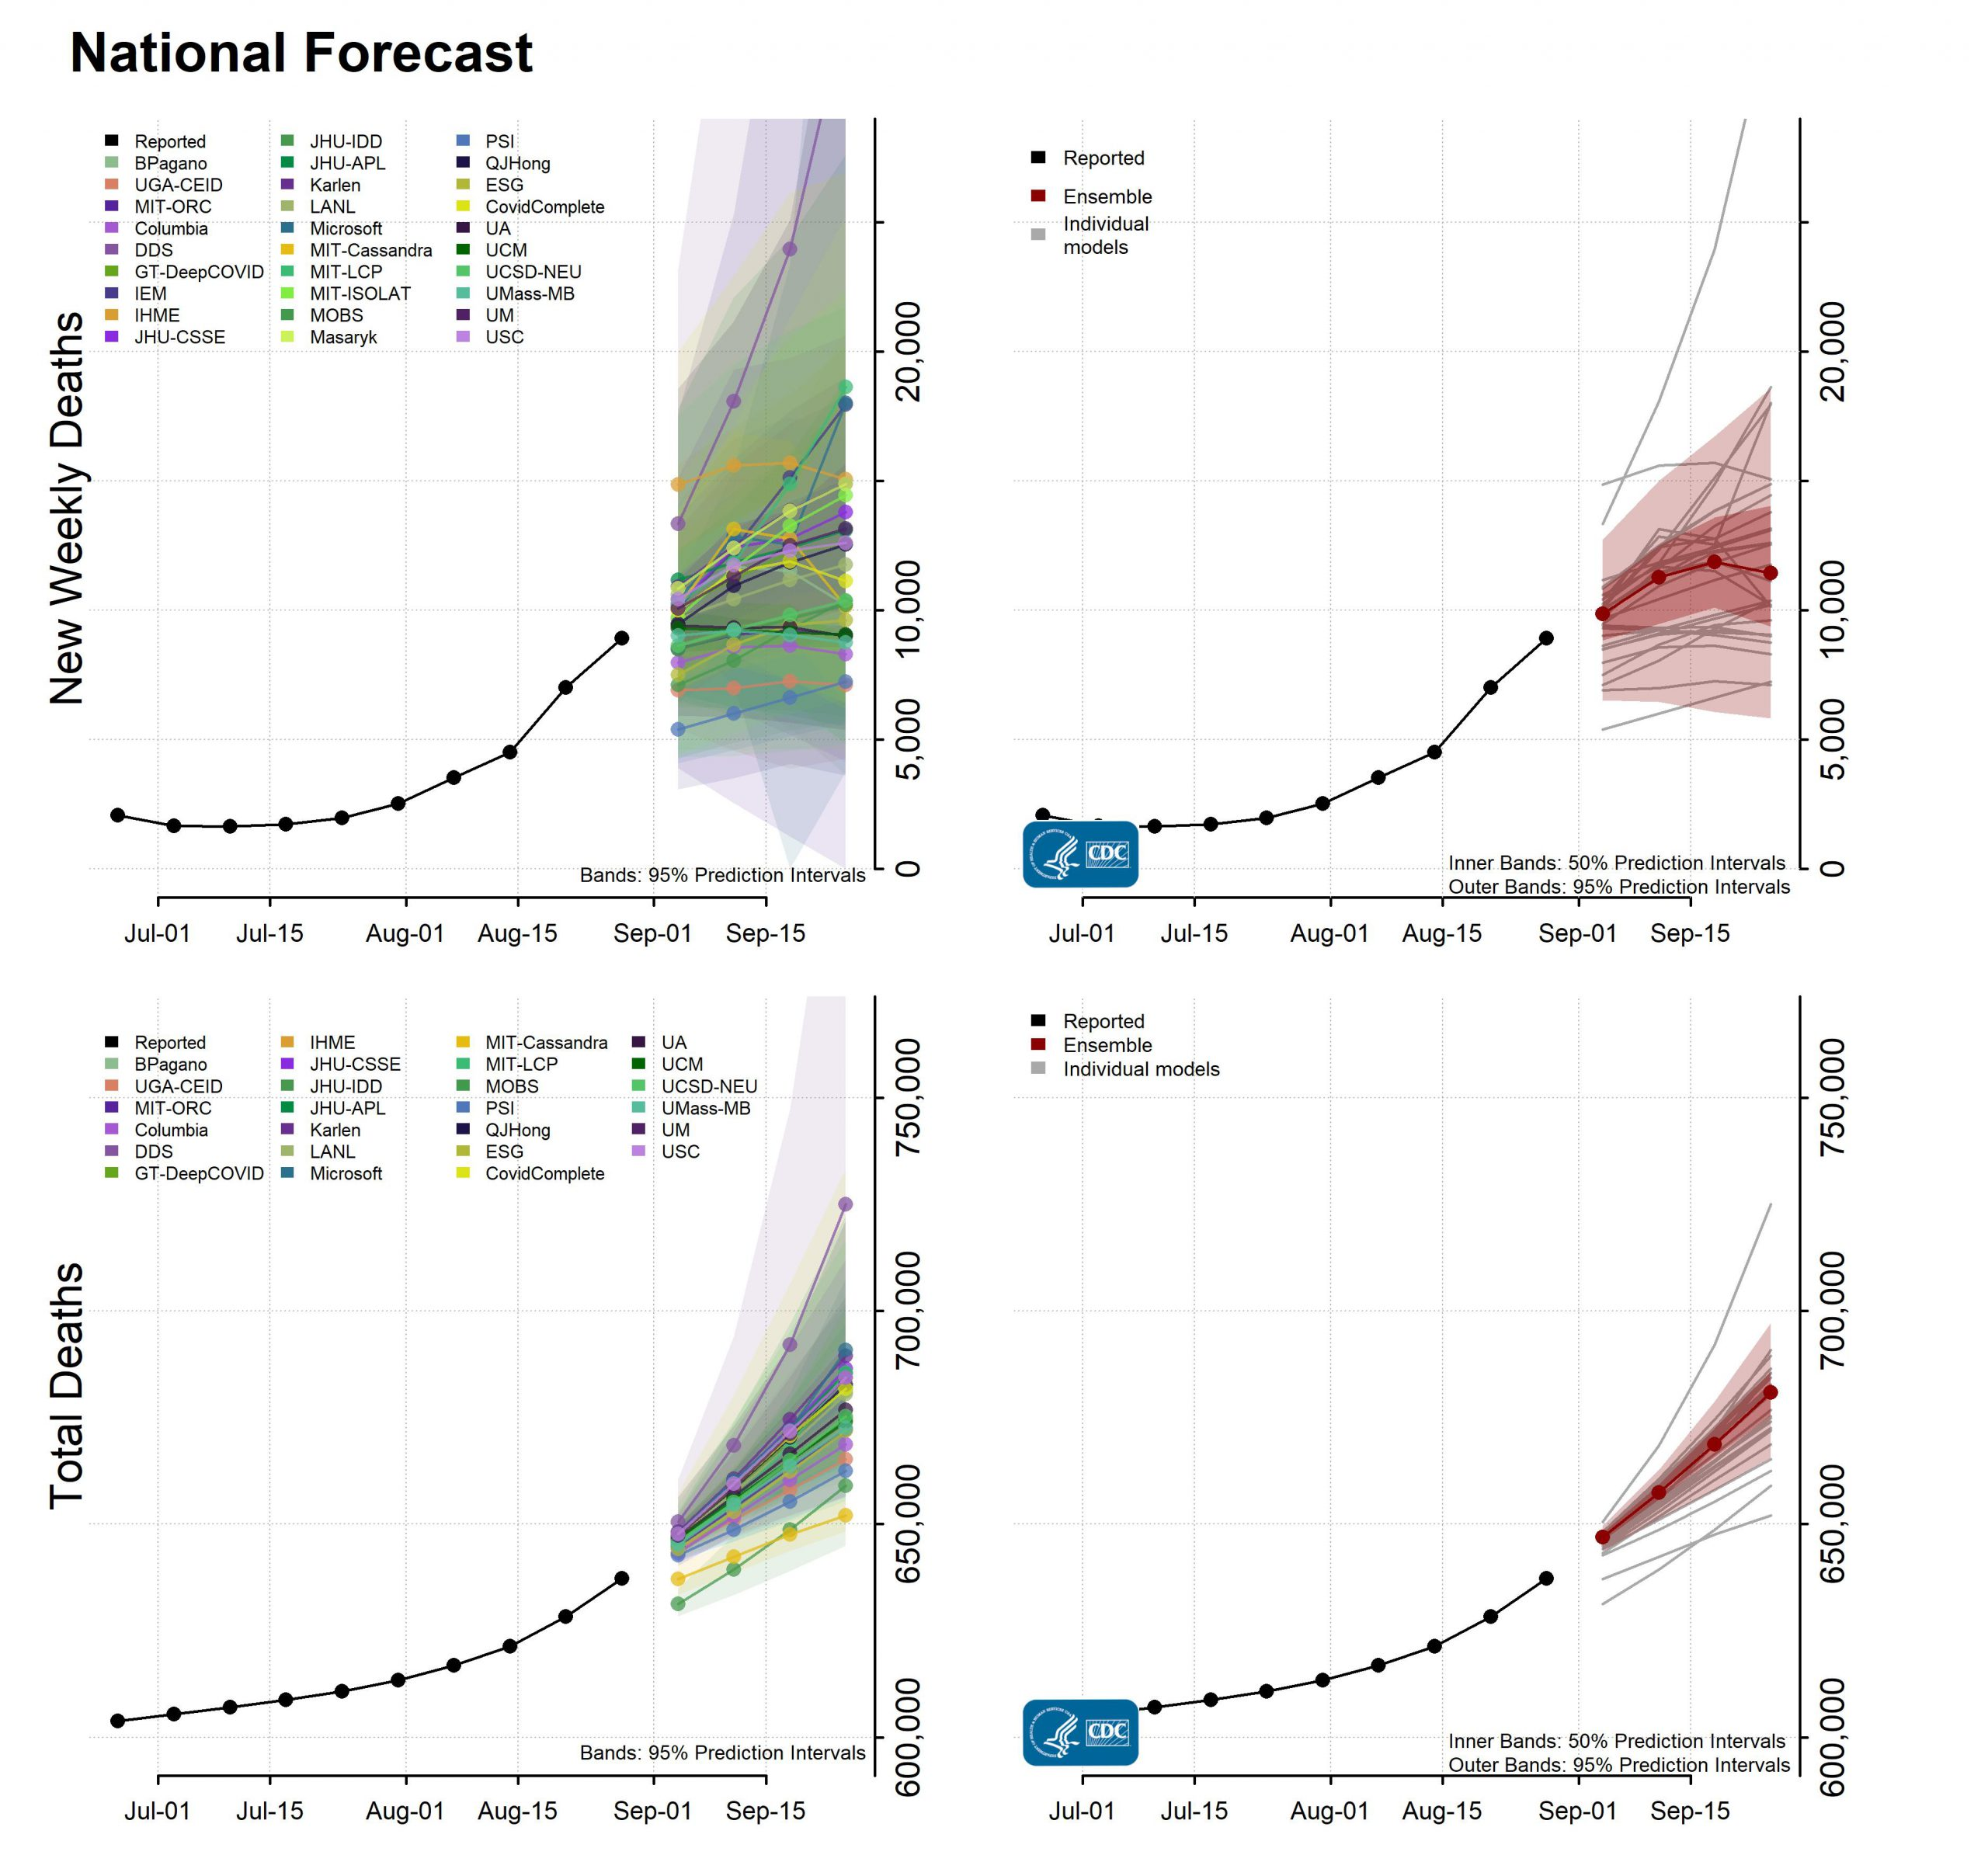
\includegraphics[scale=.12]{8_30_21_cvd_deaths.jpeg}}
\caption{Figure this out later}
\label{fig}
\end{figure}

\subsection{...}
In the context of collaborative forecasting like that of the CDC flu competition
or the COVID-19 Forecast Hub, discretized bins and quantile forecasts have 
proven useful and effective. Yet both types come with their drawbacks. Data 
storage for instance might be a concern if many bins are allowed for a 
prediction. And scoring methods are limited if forecasts are made of quantiles.

In this paper, we propose the use of discrete mixture distributions as a means 
of forecasting for projects similar to the CDC flu competition or the COVID-19
Forecast Hub. In section 2, popular probabilistic forecast representation 
types will be defined and reviewed. Methods of scoring, storing, building 
ensembles and other aspects will be reviewed and compared for each 
representation type.
Section 3 is a retrospective study of the CDC flu competition and COVID-19 
forecast predictions and an attempt to assess whether any predictions 
approximately come from well known continuous distributions.


\section{Probabilistic Forecast Representations}

Before introducing discrete mixture distributions as a candidate for a
probabilistic forecast, we review representations already commonplace in 
forecasting. In a collaborative setting, certain aspects of each representation
should be considered. With each representation presented, 
commmon application of 
scoring, data storage and ensemble construction will be considered for each type
as well as other notable properties.

\subsection{Considerations...}
\subsubsection{Scoring}
Scoring rules are used to evaluate numerically a probability forecast. The
score is a measure on the accuracy of the forecast and where multiple forecasts
exist may provide a rank for each relative to the others. If a scoring rule is 
proper, then the highest possible reward is obtained by reporting the true 
distribution. The rule is strictly proper if that value is unique. 
Under proper
scoring rules, a forecaster has no incentive to be dishonest in their 
submission \cite{gneiting2007strictly}. This makes proper scoring rules ideal
for grading forecasts. We will limit our review of scoring methods to rules
which are proper.

\subsubsection{Storage}
For a forecast hub collecting many predictions, computer storage is something
that needs to be addressed. For a project involving many researchers, the 
number of forecast predictions can add up. For example, the repository for the
COVID-19 Forecast Hub predictions contained 85.4 million predictions as of 
February 5, 2022! (cite zoltar??)
When determining the goals of a forecast project, there should be consideration 
of the storage required for different representations.

\subsubsection{Ensemble Modeling}
A multi-model ensemble is a statistical model made by combining information from
2 or more individual statistical models. Private and public decisions are 
regularly made after combining information from multiple sources. For any given
situation, information from one source may shed light on a subject which other
sources fail to capture. Likewise one statistical model may provide perspective
that another model does not, so that when they are combined in an ensemble the 
resulting model is superior.

As probabilistic forecasting becomes more commonplace, so too does ensemble 
modeling. Multi-model ensembles have been used extensively in weather and
climate modeling see \cite{baran2018combining}, 
and they have been used increasingly in modeling infectious disease outbreaks
see for example \cite{yamana2016superensemble}. 
Multi-model ensembles allow for an incorporation of multiple signals -
often from differing data sources- and for individual model biases being canceled
out or reduced by biases in others (\cite{reich2019accuracy} see references
therein). 
In several disease outbreak studies, multi-model ensemble forecasts have been 
shown to outperform individual model forecasts (\cite{cramer2021evaluation} see
references therein).

Construction of an ensemble may be done by combining individual forecast 
distributions using weighted averages. This has been called stacking 
\cite{wolpert1992stacked} or weighted density ensembles 
\cite{ray2018prediction}. 

\subsection{Representations}
\subsubsection{Parametric distributions}
A parametric distribution is a discrete or continuous probability distribution 
described by a known function $p(x) := p(x|\theta)$ -pmf in the discrete case or 
pdf in the continuous case. $\theta$ is a vector of known or unkown parameters 
contained in a parameter space. 

The value of $p(\cdot)$ evaluated at $x$ is defined as 
$p(x) = P(X = x)$ or the probability that the random variable $X$ takes
on $x$ in the space of the random variable. In the continuous case 
$P(D = x) = 0$ for all $x$, but the probability 
that $X$ falls within an interval $(a,b)$ is calculated as

\begin{equation}
  P(a < X < b) = \int_a^b p(x) dx
\end{equation}

Other functions classified by a parameteric distribution include the cumulative
distribution function (CDF) and the inverse CDF or quantile function. The CDF 
in the continuous case is defined as

\begin{equation}
  F_X(x) = P(X \leq b) = \int_{-\infty}^x p(t) dt
\end{equation}
or in the discrete case 

\begin{equation}
  F_X(x) = P(X \leq b) = \sum_{k=1}^n p(x_k) dt
\end{equation}
where $x_n$ is the largest value of X less than or equal to $x$.
The quantile function is defined as
\begin{equation}
  Q(p) = \inf \{ y \in \mathbb{R} : p \leq F_X(x) \}
\end{equation}
returning a quantile value where $p$ is a given probability $0\leq p \leq 1$.

For a forecast represented as a parametric function with pmf/pdf $p_m(x)$, 
the accuracy of the forecast may be measured as how likely realized value $x^*$
is to occur. Commonly used proper scoring rules for parametric distributions
include the Logarithmic score (LogS), 
continuous rank probability score (CRPS) \cite{hersbach2000decomposition}
\cite{alves2013ncep} and the interval/Brier 
score \cite{gneiting2007strictly} among 
others. See also \cite{gneiting2014probabilistic}
section 3 for on proper scoring functions. Unless otherwise noted, the following
definitions/reviews can be found in the review by Krueger.

For a forecast with pdf/pmf $p_m(x)$, the Logarithmic score evaluates the 
probability of the observed value $x^*$. It is defined as

\begin{equation}
  LS(p_m,x*) = -log\;p_m(x^*)
\end{equation}



 


A drawback of representing a forecast in a parametric distribution is the lack 
of flexibility in the model selection. Easy computation and evaluation of these 
models is limited to what is available in software, so certain distributional
shapes may unattainable. The distribution may assign probability to values
outside the range of the forecast. There are remedies for this such as 
truncation, but these increase the complexity in evaluation and scoring.
Requiring a parametric forecast also bars the use of some statistical methods
which might be used including certain Bayesian methods.


\subsection{Forecast as samples}
A random sample $(X_1,...,X_n)$ where $X_i \sim D$ may be used to 
estimate values such as the mean or quantiles of the distribution $D$. 

According to the Strong Law of Large numbers, the sample mean will converge to
the expected value of distribution as $n$ approaches $\infty$ as long as the 
expected value of that distribution exists. Likewise by the same law the 
empirical distribution function will converge to the true cumulative 
distribution function as $n$ approches $\infty$. Thus, if a sufficiently large 
sample is generated from a distribution, the sample will closely approximate the 
true distribution. 

For common distribution families it is easy to generate large samples using 
existing functions in R and other programming platforms. For some distributions 
for which the mathematical formula is unkown or is not in closed form, more 
sophisticated methods may be required to generate samples. Bayesian analyses may 
require a Gibbs or Metropolis-Hastings algorithm, among others, to generate a 
sample. Such samples are useful in that the true distribution may be closely 
approximated without knowing the true mathematical form. 

In the last few decades, increased computing power and improvements in MCMC
sampling have greatly contributed to growth in the use of
predictive distributions \cite{gneiting2007strictly}.

\subsection{Discretized probability bins}
A discretized bin probability distribution may be constructed over a set 
$A = [a, b]$ by partitioning $A$ into a set of $K$ bins $\{B_i\}_{i=1}^{K}$
where $B_i = [b_{i-1}, b_i)$ and $\cup_{i=1}^{K} B_i = A$. Based on the problem
to be forecasted, a forecast hub will determine the possible values for $A$ and 
select the number of bins and the sizes for each. It may the case
that a forecast hub will set the width of all bins to be equal so that 
$\Delta = b_i - b_{i-1}$ is the width for all $i$ see for example
\cite{mcgowan2019collaborative}. 
For this paper, we will consider the case where all bins share a common width.
To complete the construction, a probability $p_i$ is assigned to each $b_i$ 
where $\sum_{i=1}^{K}p_i = 1$. These probabilities are determined by the 
forecasters. 
This discrete representation with a given bin and assigned probability is in
essence a probability mass function, so a given forecast may be evaluated and 
scored the same as a discrete parametric distribution. 

If the value to be forecasted takes on discrete values, a common discrete 
distribution, such as a binary or Poisson distribution, may sometimes be used to 
assign probabilities to each of the bins. When the values to be forecasted are
continuous, a forecaster may need to employ some method of discretization to a 
forecast distribution. There are a number of possible ways to do this including
those outlined by Chakraborty and Subrata \cite{chakraborty2015generating}.
In a retroactive analysis of forecast predictions from the CDC influenza 
competition, we attempt to evaluate whether some or any teams made their 
predictions by discretizing from a common continuous distribution function.

The CDC has used a discretized distribution representation as the representation
for their annual influenza forecasting competition and other disease outbreaks.
In that context it has become the standard representation 
\cite{brooks2020comparing}. 

Most statistical models such as parametric models 
or distributions made from samples may be readily translated into a discretized 
distribution -see \cite{chakraborty2015generating} for a summary of several-
giving forecasters flexibility in how they build their 
models and assign probabilities. 
There is however some sacrifice in what can be 
forecasted as the possible range of the distribution may be limited to what the
forecast hub requires. This limitation is in part what prompted the COVID-19
Forecast Hub to use quantile forecasts rather than binned distributions.
\cite{bracher2021evaluating}.
In a simulation study outlined later, we will
consider a construction from Kemp \cite{kemp2004classes} to discretize known
continuous distributions.






\subsection{Quantile representation}
Uncertainty in a forecast prediction may also be characterized by  including
multiple quantiles along with corresponding values. Often the median value will
be reported as a point forecast with a number of quantiles included which form 
confidence intervals of various levels.
A quantile forecast is constructed as follows.
For $N$ given quantiles $\alpha_1,..., \alpha_N$, $q_1,..., q_N$ are the values
such that 

\begin{equation}
  P(Y \leq q_1) = \alpha_1, P(Y \leq q_2) = \alpha_2, ..., 
  P(Y \leq q_N) = \alpha_N
\end{equation}

When the quantiles are reported as a median and confidence intervals we have

\begin{equation}
  P(Y \leq q_1) = \alpha_1, P(Y \leq q_2) = \alpha_2, ..., P(Y \leq q_k) = .5, 
  ..., 
  P(Y \leq q_{N-1}) = 1 - \alpha_{N-1}, P(Y \leq q_N) = 1 - \alpha_N
\end{equation}

The COVID-19 Forecast Hub requires that participating teams report their
forecasts as quantile values corresponding to 23 or 7 quantiles -depending on 
the target or time being forecasted. The quantile representation was selected
over the discretized bins used in the influenza competition because the range 
of observation outcomes of interest was much larger and an appropriate binning
scheme would have been difficult to define \cite{bracher2021evaluating}.

The quantile or interval format is somewhat unique among forecast 
representations discussed in this paper. What is possible for scoring forecasts
or building ensemble models in other representations is often not possible with
quantile forecasts. Yet it has its advantages. 

Quantile representation allows for forecasters to submit fairly detailed
forecasts without restricting the range of possible values -a major reason for 
selecting a quantile representation over discretized bins 
\cite{bracher2021evaluating}. 

Since quantiles are easily calculated from any regular distribution type
-e.g. inverse CDF for parametric functions and inverse ECDF from data or 
samples- we consider quantile forecasts to have high flexbility in terms of 
shape and range. 

As in the
discretized representation, the resolution of a distribution based on quantiles
will depend on the number of quantiles to be forecasted. There is however a 
significant loss of information in reporting the extreme outcomes in a quantile
model. Since reported intervals can only be so wide, it is possible that tail 
information is lost. The COVID-19 Forecast Hub for example requires forecast 
values up to the $99^{th}$ and down to the $1^{st}$ percentile. For values any
more extreme, exactly assigning probabilities is impossible.





\subsection{Discrete mixture of parametric distributions}
In a parametric setting, forecasters may be permitted to submit a forecast as a
discrete mixture. Such a distribution may be constructed in the same way as the
ensemble described under Parametric distributions where for $T$ models with pdf
$p_t(y|\theta)$ $p^{M} = \sum_{t=1}^T z_tp_t(y|\theta)$ where 
$z_t > 0$ and $\sum_{t=1}^{T} z_t = 1$

Like the standard parametric model, a discrete mixture is easily evaluated with
exisiting software (like distr R package) (cite??) and scoring may be done by 
most or all of the same methods. The resolution of a discrete mixture is high 
and the support need not be limited by submission requirements. 

A mixture distribution may be much more flexible than a simple parametric in 
terms of distributional shape. But as it is essentially parametric, forecasters
mays still be limited in how they construct their models. But it may be possible
to fit a mixture distribution to probability models with the other 
representations discussed. Further discussion on methods for fitting mixture 
distributions to different types of model representations is included in this 
paper.

An ensemble model may be built by constructing a mixture of mixtures. Where for 
$J$ forecasts $p^{E}(y|\theta) = \sum_{j=1}^{J} w_j p^{M}_j(y|\theta)$ where 
$w_j > 0$ and $\sum_{j=1}^J w_j = 1$. (is it necessary to describe this
construction). 

Depending on the number of components a forecaster includes in a mixture 
forecast, the amount of storage per forecast might be as little as for a 
parametric forecast and as much as a forecast hub will allow.



\begin{figure}[htbp]
\centerline{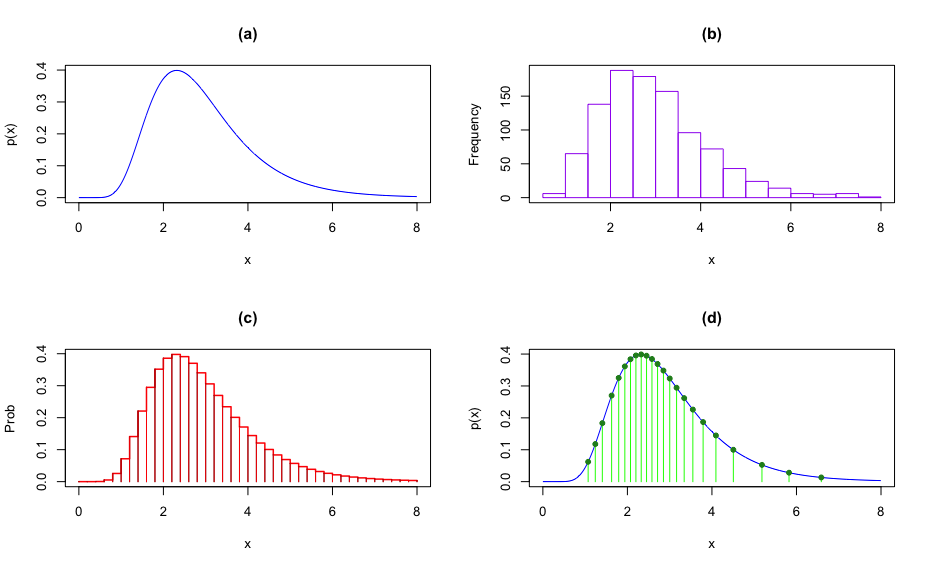
\includegraphics[scale=.4]{dens_comp.png}}
\caption{Figure this out later}
\label{fig}
\end{figure}

\begin{figure}[htbp]
\centerline{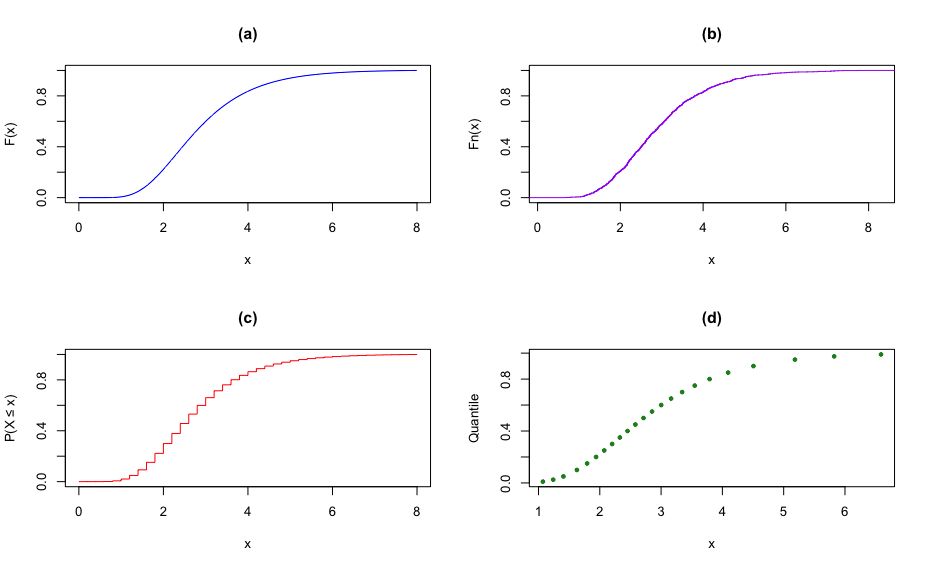
\includegraphics[scale=.4]{cum_comp.png}}
\caption{Figure this out later}
\label{fig}
\end{figure}


	 
\section{Forecast specifics on scoring, ensembling, etc.}

\subsection{Scoring}





Because the probability evaluation is only at the observed 
point \cite{reich2019accuracy} used a modified Logarithmic score 
known as the multibin logarithmic score (MBlogS) for scoring
forecasts. This allowed for a range of values to be considered "correct" or 
accurate. MGlogS is defined as

\begin{equation}
  MBlogS(F_m, y^*) = log(\sum_{i=-d}^{d} p_m(y^* + i))
\end{equation}

\begin{equation}
  \int_{y*-\epsilon}^{y^*+\epsilon} -log\;p_m(y^*) (??)
\end{equation}

The MBlogS has the advantage of offering a more accesible interpretation but the
drawback of being improper \cite{bracher2021evaluating}.

Another commonly used score, the interval score, may also be used on density 
forecasts including discretized bin forecasts. With the right smoothing of
a distribution of drawn samples, 
such as Gaussian approximation or Kernel density estimation, these methods may 
be used for scoring, see for example \cite{krueger2016probabilistic}.
These scoring methods will not work for raw samples however.

The Continuous ranked probability score (CRPS) is a function of a CDF $F$, 
including an Empirical CDF, $\hat{F}(x) = n^{-1} \sum_{i=1}^n 1\{x \geq X_i\}$
and so 
can be used a bit more extensively. For the CDF $F_m$, the CRPS is defined as

\begin{equation}
  CRPS(F_m, y^*) = \int_{-\infty}^{\infty} (F_m(y) - 1_{\{y*\leq y\}})^2 dy
\end{equation}

For a forecast of drawn samples, the ECDF may be computed and the CRPS used to 
score the prediction. The CRPS has some nice properties, but can sometimes be
difficult to compute. For example, when the forecast is a mixture of a 
Truncated Normal distribution (TN) and a Truncated Lognormal (TL) the CRPS is 
not available in closed form \cite{baran2018combining}.

The Interval score (IS), a consistent and elicitable proper score 
(see \cite{gneiting2014probabilistic} for definitions) is defined as 

\begin{equation}
  IS_{\alpha}(l,r; y^*) = (r-l) + \frac{2}{\alpha}(l-y^*)1\{y^*<l\} 
  + \frac{2}{\alpha}(y-r)1\{y>r\}
\end{equation}

where $l$ and $r$ are the $\alpha/2$ and $(1-\alpha/2)$ quantiles that bound
the central $(1-\alpha)$ prediction interval. This is a sum -weighted by 
$\alpha$- of the width of the
interval and the distance between $y^*$ and the interval (if $y^*$ is not 
captured in the interval). The IS requires only a single central 
$(1-\alpha) \times 100$ prediction interval.

When an interval forecast is made up of more than one interval with different
$\alpha$ levels, a weighted interval score (WIS) may be evaluated. Bracher et.
al use the WIS to evaluate COVID-19 inverval forecasts 
\cite{bracher2021evaluating}. There are multiple versions of the WIS -some of 
which are described by Bracher et. al- but that used in the COVID-19 Forecast
Hub is defined as follows.

\begin{equation}
  WIS_{0,K}(F_m,y^*) = \frac{1}{K + 1/2} \times (w_0, \times |y^*-med|+
  \sum_{k=1}^K \{ w_k \times IS_{\alpha_k}(F_m,y) \} )
\end{equation}

where $F_m$ is the interval forecast, $K$ is the number of prediction intervals
each with level $\alpha_k$ and $med$ is the predictive median. $\alpha_0 = 1$ is 
is the $\alpha$ value corresponding to the predictive median which may also be
considered a level 0 prediction interval. $w_k = \alpha_k/2$ is the weight on
intervals which was used. With that choice of weights, it may be shown that the
WIS approximates CRPS see S1 Text  \cite{bracher2021evaluating} or

\begin{equation}
  WIS_{0,K}(F_m,y^*) \approx CRPS(F_m,y^*)
\end{equation}

Bogner, Liechti and Zappa compared scoring forecasts of quantiles with the 
Quantile Score similar to the interval score and scoring distribution functions
fit to those quantiles using CRPS \cite{bogner2017combining}. The CRPS 
corresponds to the integral of the QS over all possible thresholds rather than
just specific quantiles, it more effectively reveals deficiencies in parts of 
the distribution and especially in the tails past the end points of quantiles
used in QS or IS.





\subsection{Flexibility, resolution and information (such as tail info)}
The amount of info


\subsection{Ensemble}


Considered the state-of-the-art techniques for combining component distributions
into a multi-model ensemble are nonhomogeneous regression (NR), also known as
ensemble model output statistics (EMOS), and ensemble Bayesian model averaging
(BMA), both of which will be defined as in \cite{gneiting2014probabilistic}.

In the context of an ensemble made from component models submitted from various
sources, contructed with different methods and with potentially different data,
BMA is the better option. In BMA, the final model does not have to be specified
beforehand and the resulting forecast will be a discrete mixture distribution
of all component forecasts. The general form for the ensemble distribution $p^E$
is

\begin{equation}
  p^E(y) = \sum_{j=1}^J w_jp_j(y)
\end{equation}
where $p_j$ is the $j^{th}$ component forecast distribution and 
$0 \leq w_j \leq 1$ is a weight assigned to each component where $\sum w_j = 1$.
Methods for estimating weights include Maximum Likelihood estimation
\cite{raftery2005using}, MCMC 
sampling see \cite{vrugt2008ensemble} (also in this paper it talks about how 
EM can get difficult as parameters i.e. number of distributions increase, and 
shows MCMC may be better with that high dimensionality and gives full posterior
of weights)
and minimizing CRPS as in 
\cite{baran2018combining}.

Reich et. al used BMA to combine multiple forecasts from the flu 
competition. There built and compared ensemble models with different weighting
schemes including equally weighted components $w_j = 1/J$ and estimating weights
according to the model specification. To estimate weights they used the 
Expectation Maximization (EM) algorithm \cite{reich2019accuracy}. See the
supplementary material for details. Other options for estimating the weights 
include Monte Carlo Markov Chain sampling ??\cite{vrugt2008ensemble} or a 
minimization of the ensemble CRPS score \cite{baran2018combining}.

The BMA ensemble construction works for discrete and continuous parametric 
distributions as well as discretized bin distributions, but is not useful when 
the forecasts are of the interval type. 

Quantile averaging or Vincentization is defined as 

\begin{equation}
  F_v^{-1}(\alpha) = \sum_{m=i}^M w_m F_m^{-1} (\alpha)
\end{equation}

where $F_m^{-1} (\alpha) = \inf \{y:F_m(y) \geq \alpha\}$ for 
$0 < \alpha \leq 1$. Some notable characteristics are that it is more likely
to be unimodal than linear averaging of densities like BMA 
\cite{busetti2017quantile} (this paper is a big comparison of QMA and 
linear or log averaging. Under some circumstances, such as when member
distributions are exponential, Weibull or logisitic the aggregated distribution
is the same \cite{ratcliff1979group}. It apparently produces smoother
distributions than BMA, at least in \cite{schepen2015model}.

These dudes seem to think averaging quantiles is better than simple averaging 
probabilities. More sharp (less variation), perform better in scoring etc.
\cite{lichtendahl2013better}.


\subsection{Storage}


The data requirement for a parametric distribution small and will usually be the 
least when compared with other representations. As long as the forecast is 
allowed to have an unbounded range, only 3 or 4 pieces of information will be
required including specification of the distribution family and model 
parameters. See the table below for an example of a normal distribution with 
mean 0 and variance 1.

\begin{table}[h!]
\centering
 \begin{tabular}{||c c c c||} 
 \hline
 Family & param1 & param2 & param3 \\ [0.5ex] 
 \hline\hline
 lnorm & 1 & 0.4 & NA \\ 
 \hline
 \end{tabular}
\end{table}

With those three pieces of information, the whole distribution is completely
defined and software is readily available for calculating moments, percentiles,
probabilities and generating random samples. The third box under param3 is there
in case a particular distribution family has three parameters -a location-scale
T distribution for example.

If the distribution is made up of samples from a distribution, like posterior
predictive distribution, much more space will be required to contain all the 
information. A sample using MCMC sampling may have thousands or even tens of 
thousands of draws. It's easy to see why this could be a problem if millions of
predictive distributions are collected and saved.

The exact amount of information required for a discretized bin forecast will 
vary depending on permitted range of the forecast and the desired resolution. 
In the CDC flu contest, a forecast could have 131 bins between 0\% and 13\% 
-bins having increments of 0.1- with 
corresponding probabilities in each. That makes 262 pieces of information per
prediction. A much larger number than what is required for a fully defined
parametric distribution. The following table shows what a discretized standard
normal distribution looks like in 131 discretized bins. Note that for the sum of 
the probabilities to equal one, it was essential to normalize the probabilites
within the range $[-6.5,6.5]$ since the full range of a normal distribution is
$(-\infty, \infty)$.

\begin{table}[h!]
\centering
 \begin{tabular}{|c|c|} 
 \hline
    bin & prob \\ \hline
    ... & ... \\
    {[1.4,\;1.6)} & 0.04414 \\
    {[1.6,\;1.8)} & 0.05896 \\
    {[1.8,\;2.0)} & 0.07032 \\
    {[2.0,\;2.2)} & 0.07172 \\
    {[2.2,\;2.4)} & 0.07955 \\
    ... & ... \\
 \hline
 \end{tabular}
\end{table}

Like in the last two representations, data storage for interval forecasts will
depend on the desired clarity of resolution. For the COVID-19 forecasts 
submitted to the forecast hub, twenty-three quantile values are requested for 
the quantiles (0.01, 0.025, 0.05, 0.10, …, 0.95, 0.975, 0.99). This included a 
median along with eleven confidence intervals \cite{bracher2021evaluating}. This
requires forecasters to submit forty-six values in each short-term forecast 
(some of the longer term forecasts only include seven quantiles). In terms of 
storage, this is an improvement over requirements for the flu contest. 


\begin{table}[h!]
\centering
 \begin{tabular}{|c|c|} 
 \hline
    quantile & value \\ \hline
    0.01 & 1.07137 \\
    0.025 & 1.2404 \\
    0.05 & 1.40689 \\
    0.01 & 1.62675 \\
    ...  & ... \\
    0.9 & 4.50667 \\
    0.95 & 5.18328 \\
    0.975 & 5.82391 \\
    0.99 & 6.58783 \\
 \hline
 \end{tabular}
\end{table}


\begin{flushleft}
    \begin{adjustwidth}{-3cm}{-1cm}
    \begin{tabular}{ | p{2.4cm} | p{2cm} | p{4cm} | p{3cm} | l |}
    \hline
    Representation & Scoring & Flexibility/Information & Ensemble &
    Storage Requirement
    \\ \hline

    Parametric & All methods & Limited to common distribution families 
    &  & Low 3-6 values \\ \hline
    
    Discretized bins & All methods, more computation required for some (CRPS) &
    Any shape allowed, but limited to bin description and range & &
    High
    \\ \hline

    Samples & Limited to CRPS and IS unless smoothing is performed & High & & 
    Very high, thousands of values
    \\ \hline

    
    Quantiles & IS, WIS & High & & Medium 
    \\ \hline
    
    Discrete Mixture & All methods, but may be limited by computation & 
    High with proper approximation &
    & Low-Medium
    \\ \hline

	 \end{tabular}
	 \end{adjustwidth}
\end{flushleft}

% bin & -6.5 & -6.4 & -6.3 $ ... & 6.3 & 6.4 & 6.5 \\  
%  prob & 3.75e-11 & 1 7.11e-11 & 1.33e-10 & ... & 7.11e-11 & 3.75e-11 & 1.96e-11\\

\newpage


\section{Retrospective Analysis}

\subsection{CDC Influenza like Illness}
The CDC Retrospective Forecasts project at zoltrdata.com (cite??) contains over
850,000 probabilistic ILI predictions for all combinations of of eleven regions 
in the United States and seven targets from twenty-seven different models. These
include predictions during Influenza season between October 2010 and December
2018. All predictions are in the form of discretized probability bins. 

We wanted to determine whether or not some or any of these binned forecasts may
have come from known continuous distribution families such as Uniform, Normal, 
Lognormal or Gamma families. The process we followed for making such a claim was
to "fit" a distribution to the probabilities provided in the forecast by
minimizing

\begin{equation}
  \sum_{i=1}^K (p_i - [F(b_i; \theta) - F(b_{i-1}; \theta)])^2
\end{equation}

Here $F(\cdot; \hat{\theta})$ is a CDF, $p_i$ is the reported probability for 
the $i^{th}$ bin $B_i := [b_{i-1}, b_i)$ and $K$ is the number of bins.
The fitted parameter vector $\hat{\theta}$ is the solution to 

\begin{equation}
\arg\min_{\theta}\sum_{i=1}^K (p_i - 
[F(b_i; \theta) - F(b_{i-1}; \theta)])^2
\end{equation}

If well known continuous distribution was fit to the submitted binned prediction
and the mean sum of squared differences fell below a specified cutoff value, we
considered that the binned predictions were plausibly discretized from the 
continuous distribution.


To determine what values to use as cutoffs we conducted a study where 
binned distributions were discretized from known continuous distributions, 
parameters were fit to the binned distrubtions and the mean sum of squared 
differences was calculated.

For each of Uniform, Truncated Normal (TN), Truncated Lognormal (TL) and 
Truncated Gamma (TG) distributions the following was
done 1,000 times. A set of 131 bins with interval lengths of 
0.1 between 0 and 13.1 was constructed. 
A value $\mu$ was selected from a $Uniform(a,b)$ distribution and $\sigma$ from 
a $Uniform(.05,1.6)$ distribution. $\mu$ and $\sigma$ were taken as respectively 
the center and scale parameters of a TN distribution. 
For Uniform, TL and TG family
distributions, model parameters were solved for so that $\mu$ and $\sigma$ 
were roughly the mean and standard deviation. The minimization was done using 
the `optim` function in the R `stats` package.
Had we accounted for the changes
in moment values from the truncation, the means and standard deviations could 
have been exactly $\mu$ and $\sigma$. But we considered the differences small 
enough that it didn't matter for our purpose.

With a known distribution, probabilities $p_i =F(b_i; \theta) - F(b_{i-1})$ were
calculated for each bin. A Uniform or truncated distribution from the same
family was fit to the bins by minimizing (equation number) with the resulting
distribution function $F(\cdot; \hat{theta})$. From the fitted distribution
$\hat{p_i} = F(b_i; \hat{\theta}) - F(b_{i-1}; \hat{\theta})$ was computed for 
each of the 131 bins. Finally the mean sum of squared probability differences
$\frac{1}{K}\sum_{i=1}^K (\hat{p_i} - p_i)^2$ was calculated. Table (table number)
below shows MSD value for which 95\% of all 1,000 MSDs fell below. Other than in
the case of the Uniform distribution family, those values were selected as the 
cutoff values for declaring whether or not a binned distribution was discretized
from a common continuous distribution.


\begin{table}[h!]
  \centering
  \begin{tabular}{l*{6}{c}r}
  Distribution          & Mean Square Difference 95\%  \\
  \hline
  Uniform               & 8.809460e-05   \\
  Truncated Normal      & 1.126683e-07  \\
  Truncated Lognormal   & 3.877829e-06  \\
  Truncated Gamma       & 1.500152e-06  \\
  \end{tabular}
\end{table}




Of the 869,638 predictions from the CDC Retrospective Forecast project, we fit
each of Uniform, TN, TL and TG distributions to 11,715 of the individual 
predictions. The MSD between the prediction probabilities and the fit
discretized probabilities was calcuated. For each prediction, the fitted 
distribution with the lowest MSD was considered the best fit and if the MSD fell
below the corresponding cutoff value listed in (table number) we consider that 
the prediction approximately follows the fit distribution. The results for the
11,715 fit distributions are seen below.

\begin{table}[h!]
  \centering
  \begin{tabular}{l*{6}{c}r}
  Distribution Family   & Total    & Total Below MSD Cutoff \\
  \hline
  Uniform               & 896      & 669    \\
  Truncated Normal      & 3,804    & 198    \\
  Truncated Lognormal   & 4,501    & 1,340  \\
  Truncated Gamma       & 2,514    & 295    \\
  \end{tabular}
\end{table}

\subsection{COVID-19 Forecast Hub}

As of January 24, 2022 there were nearly 85,000,000 prediction distributions 
from 114 different models submitted to the COVID-19 Forecast Hub (cite??). These 
distributions covered all combinations of 3,202 municipalities (mostly counties) 
in the United States with 441 targets. The first of these forecasts was 
submitted in March of 2020 shortly after the initial outbreak of the virus in 
the US and forecasts had been received weekly since. The forecast representation
for these predictions is the quantile representation where a point estimated is
submitted along with a number of confidence intervals -three or eleven for most
targets. So the predictions typically include seven or twenty-three quantiles.

To assess whether or not a quantile based forecast was formulated from a well
known continuous distribution, we minimized the MSE between the cumulative
density function and the given quantiles. The estimated parameters are the 
solution to $argmin_{\theta} \sum_{i=1}^m (q_i - F(y; \theta))$ where $q_i$ is
the $i^{th}$ given quantile value and $F(y; \theta)$ is the CDF with parameter
$\theta$. This least squares estimating is a more common way to fit a model but
other methods have been presented including Bayesian Quantile Matching
\cite{nirwan2020bayesian}, step interpolation with exponential tails 
\cite{quinonero2005evaluating}
and the Method of Simulated Quantiles 
\cite{dominicy2013method}.

For each prediction used, we fit the quantiles to a Uniform, Normal, Lognormal,
Gamma and Location-scale T CDF. We included the T distribution in case of any
symmetric forecasts with tails heavier than in a Normal distribution.

If the MSE between a given forecast and a fit CDF fell below a certain cutoff,
we considered the quantiles as approximately coming from the fit CDF. To
determine the cutoff values, for each of the five distribution families the same
procedure was followed 1,000 times. 

A decision was made on creating a quantile distribution with 7 quantiles or 23
quantiles with probabilities 1/3 and 2/3 respectively. This was done because 
in the COVID-19 Forecast Hub certain targets require 7 quantiles and others 
require 23. After that decision was made, a random value $\mu$ was drawn from
a $Uniform(2,000,\; 25,000)$ distribution and another value $\sigma$ was drawn
from a $Uniform(3, 200)$ distribution. These values were taken as the mean and
standard deviation and for each of the distribution families considered, the
proper transformations computed to find model parameters corresponding to the 
distribution. Quantile values were calculated for each quantile. When using an 
LST distribution, a value for degrees of freedom was drawn from a 
$Uniform(2,35)$ distribution. A CDF
was fit by minimizing $\sum_{i=1}^m (q_i - F(y; \theta))$ over the parameter
vector $\theta$ and the MSD value $\sum_{i=1}^m (q_i - F(y; \hat{\theta}))$ was 
calculated. The MSD value for which 95\% of the 1,000 simulated distributions
fell below was considered the cutoff and is seen in the table below.

\begin{table}[h!]
  \centering
  \begin{tabular}{l*{6}{c}r}
  Distribution          & Mean Square Difference 95\%  \\
  \hline
  Uniform               & 7.220667e-07   \\
  Normal                & 3.097645e-05  \\
  Lognormal             & 1.166775e-07  \\
  Gamma                 & 2.953370e-05  \\
  Location-scale T      & 0.4894471 \\
  \end{tabular}
\end{table}


With these cutoff values selected, models were then fit to quantile forecasts
from the COVID-19 Forecasts on zoltardata.com. This was a computationally more
difficult problem than fitting distributions to the binned forecasts of the 
influenza project, so the number of predictions fit is much smaller. The 
predictions fit were selected from each of the 115 models with model weeks, 
targets and units selected randomly. In total 2,504 predictions were fit to each
of the five distributions, the MSE was calculated for each and the fit with the
lowest MSE was selected as the closest fit. If the MSE fell below the cutoff
specified above, we considered that the quantile prediction was approximately
from the same distribution as the fit distribution. The results are below.


\begin{table}[h!]
  \centering
  \begin{tabular}{l*{6}{c}r}
  Distribution Family   & Total    & Total Below MSD Cutoff \\
  \hline
  Uniform               & 239      & 0        \\
  Normal                & 609      & 74       \\
  Lognormal             & 694      & 0        \\
  Gamma                 & 597      & 0        \\
  Location-scale T      & 365      & 25       \\
  \end{tabular}
\end{table}



















\newpage 

\section*{everything below here is just notes for now}


Even as computing power and memory storage continue to improve, 
A single probabilistic forecast can range from only a few pieces of data, such 
as a well known distribution family and two given parameters, to thousands or
tens of thousands of MCMC draws from a posterior distribution. When a repository
of forecasts contains many millions of individual prediction distributions, such
as the COVID-19 Forecast Hub \cite{Cramer2021-hub-dataset}, large file type forecasts can become a 
problem. (Say something about MechBayes posterior samples vs. quantile version
of the forecast).
Something about ensemble storage...





Bogner, Liechti and Zappa compared scoring forecasts of quantiles with the 
Quantile Score similar to the interval score and scoring distribution functions
fit to those quantiles using CRPS \cite{bogner2017combining}. 
The CRPS proves more effective than QS in 
revealing model issues especially in the tails.

Depending on the forecast representation, certain scoring rules may not work to 
assess a forecast. For example, for a quantile or interval representation, LogS
and CPRS may not be used. The weighted interval score was used by Bracher et. al
to evaluate forecasts collected by the COVID-19 Forecast Hub. 
\cite{bracher2021evaluating}







As the number of quantiles required increases, so does the per forecast storage 
requirment. In the COVID-19 Forecast Hub, $23\times 2 = 46$ pieces of 
information are required for certain targets. And because quantiles are easily 
obtained from most methods of probabilistic modeling, teams have much 
flexibility in the type of modeling they perform. 

Ensemble modeling under quantiles is done by averaging each quantile over all 
forecast models. Weighting the models based on past performance may be done, but
may not always prove worth the effort. (cite??) A shortcoming of quantile
averaging is the limit that ensemble distributions shapes may take. It has been
shown that quantile averaging may only produce quantiles for distributions which
are unimodal. (cite??) Another shortcoming is that not all proper scoring
methods are appropriate in scoring quantile forecasts. The log-score may not be 
used for example. There are, however, alternatives for scoring such as the
weighted interval score. (cite??)

\subsection*{Above quantiles below bins}

Thus point estimates and
probabilities are easily calculated and proper scoring of each forecast may be 
done with the usual methods. 

To build an ensemble forecast from several individual forecasts, each bin may be
averaged over all forecasts. This may be done with or without weighting of the 
various models and the weights if selected may be assigned using the same 
methods that may be used for parametric distribution forecasts.

The discretized representation can provide distributions with reasonably high
resolution but with some cost. As the width of the bins decreases, the 
resolution increases but the storage increases. The number of bins may range 
from a few dozen to hundreds requiring just as many rows in a data table and at 
least two columns. The CDC for example reuqired participants to submit 
probabilities for 51 bins per forecast in the influenza forecasting competition. 
Each team then, had to submit $51\times2 = 102$ pieces of information.

\subsection*{Above bins, below pdfs}


Where a forecast hub requests a parametric distribution as a forecast, a 
submission of three or four cells of data per forecast may suffice making this
representation very efficient for storage. (See table ??)
That little information is enough to provide a high resolution forecast over
all possible values of the forecast. Evaluation of parametric forecasts may be 
done using most proper scoring methods such as the log-scoring method
\cite{gneiting2007strictly}
or modifications of the log-scoring method such as that used by the CDC in 
influenza forecasting \cite{reich2019collaborative}.

In building an ensemble forecast, a discrete mixture distribution may be used.  
To construct a mixture distribution suppose there are $J$ forecasts represented
by parametric distributions with probability density functions $p_j(y|\theta)$ 
for $j = 1,..,J$. A mixture distribution of the $J$ forecasts is 

$$p^{E}(y|\theta) = \sum_{j=1}^{J} w_j p_j(y|\theta)$$
where $w_j > 0$ and $\sum_{j=1}^{J} = 1$ are weights assigned to each to each 
component. Equal weights may be assigned to each forecast so $w_j = 1/J$ for all
$j$ or they may be determined by the accuracy and precision of the individual
forecast. Bayesian model averaging \cite{raftery2005using}
is one reasonable way to select weights, though there are 

A drawback of representing a forecast in a parametric distribution is the lack 
of flexibility in the model selection. Easy computation and evaluation of these 
models is limited to what is available in software, so certain distributional
shapes may unattainable. The distribution may assign probability to values
outside the range of the forecast. There are remedies for this such as 
truncation, but these increase the complexity in evaluation and scoring.
Requiring a parametric forecast also bars the use of some statistical methods
which might be used including certain Bayesian methods.

\begin{table}[h!]
\centering
 \begin{tabular}{||c c c c||} 
 \hline
 Family & param1 & param2 & param3 \\ [0.5ex] 
 \hline\hline
 normal & $\hat{\mu}$ & $\hat{\sigma}$ & NA \\ 
 lst & $\hat{\mu}$ & $\hat{\sigma}$ & $\hat{\nu}$ \\ [1ex] 
 \hline
 \end{tabular}
\end{table}

 



\subsection*{Information}
	 

	 

\newpage    
\bibliographystyle{apacite}
\bibliography{references}
\end{document}


